\section{Contexte}

Ce projet vise à concevoir un système mesurant le temps de réaction d'un utilisateur à un stimulus visuel, avec une précision d'une milliseconde. L'utilisation du système d'exploitation FreeRTOS garantit le respect de ces contraintes de temps strictes. \\

Le matériel se compose d'une carte SAMD21XPLAINEDPRO et de son extension OLED1XPLAINEDPRO (écran, LEDs, boutons), programmées sur Microchip Studio. Ce rapport explique l'intégration de FreeRTOS, détaille l'architecture logicielle (tâches, sémaphores) et valide le bon fonctionnement du système.

\begin{figure}[H]
    \centering
    \begin{subfigure}[b]{0.48\linewidth}
        \centering
        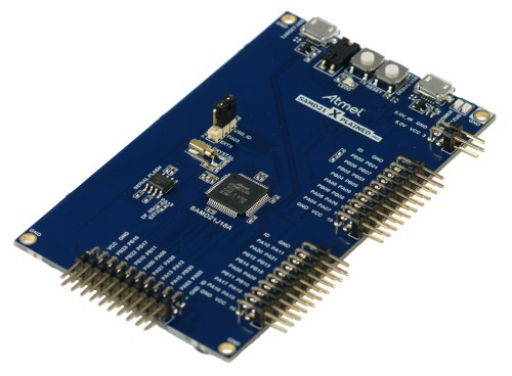
\includegraphics[width=\linewidth]{Figures/sam d21 xplained pro evaluation.png}
        \caption{Carte SAMD21XPLAINEDPRO}
        \label{fig:carte_SAMD21XPLAINEDPRO}
    \end{subfigure}
    \hfill
    \begin{subfigure}[b]{0.48\linewidth}
        \centering
        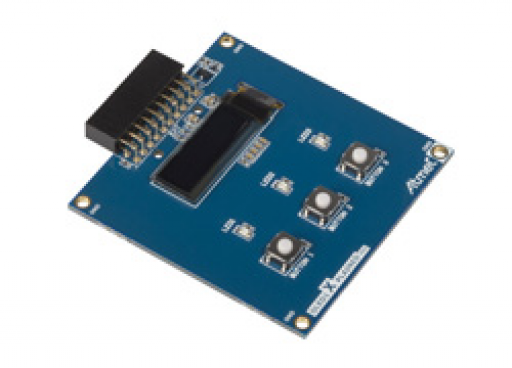
\includegraphics[width=\linewidth]{Figures/oled1 xplained pro extension kit.png}
        \caption{Extension OLED1XPLAINEDPRO}
        \label{fig:extension_OLED1XPLAINEDPRO}
    \end{subfigure}
    \caption{Matériel utilisé pour le système de mesure du temps de réaction}
    \label{fig:materiel_systeme}
\end{figure}